\documentclass[a4]{article}
\usepackage{graphicx}

\addtolength{\textwidth}{5cm}
\addtolength{\textheight}{5cm}
\hoffset-3cm
\voffset-3cm

\begin{document}
\section{Basic examination and processing}
Within this strand of work we are looking at the GPS and IMU data from
the RC car ``long trajectories'' in Stanmer Park. The overall goal is to
examine this data, clean up any issues in it and make it ready for
working on assessing visual navigation algorithms.

First, we examine the data by plotting the x and y cordinates of GPS
locations taken along the 15 trajectories. The data is plotted in
figures \ref{fig:rawTraj1} to \ref{fig:rawTraj2}.

The first basic observations are:
\begin{enumerate}
  \item It looks like the coordinates are in m - not in mm as
    stated in the csv files. If true, the trajectories are some $700$m
    or so long. I will describe everything below under the assumption
    of units being m.
  \item The trajectories start with the vehicle standing still but we
    can see some drift. Some trajectories have more, some less but on
    the order of tens of cm (see figure \ref{fig:rawTrajDetail}.
  \item The trajectories presumably started at the same physical
    location but the recorded starting positions appear offset between
    trajectories by on the order of $4-8$ m. Furthermore, normalising
    them to start from the same location does visually not seem to
    improve the overlap of trajectories, suggesting it is not just a
    global offset between them (see more about this below)
  \item The end of the trajectories is fairly inconsistent, see also
    figure \ref{fig:rawTraj2}. To do meaningful comparisons of visual
    navigation algorithms between trajectories, it appears sensible to
    cut the trajectories to a 
    common, fairly consistent part.
\end{enumerate}

\begin{figure}
  \includegraphics[width=
    \textwidth]{figures/raw_trajectories_onepanel.png}
  \caption{\label{fig:rawTraj1} Trajectories as recorded by GPS
    without any processing applied. All 15 datasets are shown.}
\end{figure}

\begin{figure}
  \includegraphics[width=
    \textwidth]{figures/raw_trajectories_onepanel_detail.png}
  \caption{\label{fig:rawTrajDetail} Detail of previous figure focussing on
    the trajectory start.}
\end{figure}

\begin{figure}
  \includegraphics[width=
    \textwidth]{figures/raw_trajectories_manypanel.png}
  \caption{\label{fig:rawTraj2} Trajectories as recorded by GPS
    without any processing applied. All 15 datasets are shown. Mainly
    included here to be able to identify trajectories and the
    corresponding data set names.}
\end{figure}

Based on the observations I have made the following first processing
steps (\verb+zero_chop.py+):
\begin{enumerate}
  \item Remove the initial non-moving phase: Here I removed all points
    where the car did not move more than \verb+min_move+ m within
    \verb+pt_dist+ data points (or the next non-NaN point if that is a
    NaN point). For now I have used \verb+min_move+$= 0.5$ m and
    \verb+pt_dist+$= 20$.
  \item Remove any part of the trajectory once the $y$ coordinate has
    passed below $5638423$ for the first time. This cut-off was chosen
    by eyeballing the common part of all trajectories.
\end{enumerate}
The resulting trajectories are shown in figure \ref{fig:procTraj1}.
\begin{figure}
  \includegraphics[width=\textwidth]{figures/cut_trajectories_onepanel.png}
  \caption{\label{fig:procTraj1} Minimally processed trajectories with
  initial non-movign phase cut and everything byond the stated $y$
  threshold cut.}
\end{figure}

\begin{figure}
  \includegraphics[width=\textwidth]{figures/cut_trajectories_samex0y0_onepanel.png}
  \caption{\label{fig:procTraj2} Same a previous figure but with the
    initial position of the initial trajectory subtracted. Note how
    these do {\em not} appear to overlap better.}
\end{figure}

Before doing any more analysis, it is very inconvenient that about
every third GPS position is recorded as NaN. This is presumably due to
some mismatch of recording frequencies for GPS and other data and
other GPS failures (there are also larger gaps at (thankfully) rare
times). Also, there is some obvious noise in the GPS readings. To get
somthing more consistent I have taken an approach of fitting pieces of
the trajectory with a polynomial function and recombining all fitted
pieces by averaging to one interpolated trajectory. This is done with the script
\verb+fit_trajectories.py+. For now, I have included results with
polynomial degree $1$ (simple linear regressions) and on pieces of
trajectory of $75$ data points each.

Next, we examine the heading information from fitted trajectories and
from the IMU recordings. There are jumps in the IMU recordings, which
are some kind of artefact of unknown origin. I was not able to find a
simple explanation (such as power outage, with reset to 0 or such). I
have removed these jumps by the following method (\verb+correct_heading.py+):
\begin{enumerate}
  \item Whenever the heading reading of the IMU jumps by more than 15
    degrees in a single timestep, the jump is subtracted from the
    subsequent headings.
  \item I shift the heading data globally so that the average IMU
    heading matches the average GPS-based heading. GPS-based heading
    was calulculated simply based on straight line connections between
    subsequent data points on the interpolated GPS trajectory.
\end{enumerate}
Figure \ref{fig:correctHeading} shows the results. The original IMU
data, also shifted to match means, is shown in blue, the corrected IMU
data in orange and the GPS derived heading in green. The match is
arguably sensible even though not perfect. For one, the GPS heading
seems to undershoot in sharp turns. This could potentially be improved
by taking less points for the trajectory regressions or a higher
degree of the fitted polynomials. There are also a couple of sections
in individual trajectories where the match is slightly less good.

To give a better impression of the quality of the fitted trajectory
and heading fit, I have made movies that move a ``magnifying glass''
along the trajectories and display the original GPS locations, the fitted trajecory points and GPS derived and IMU derived headings
(as a quiver plot).
(\verb+make_movie_frames.py+ and then using \verb+ffmpeg+ like so:
\verb+>> ffmpeg -framerate 10 -pattern_type glob -i "frame_*.png" output.mp4+),

\begin{figure}
  \includegraphics[width=\textwidth]{figures/corrected_heading.png}
  \caption{\label{fig:correctHeading} Heading
  shown as a function of time. For the purposes of this plot I have
  ``unrolled'' the angle so that there are no ``jumps'' of 360 degree.}  
\end{figure}

\begin{figure}
  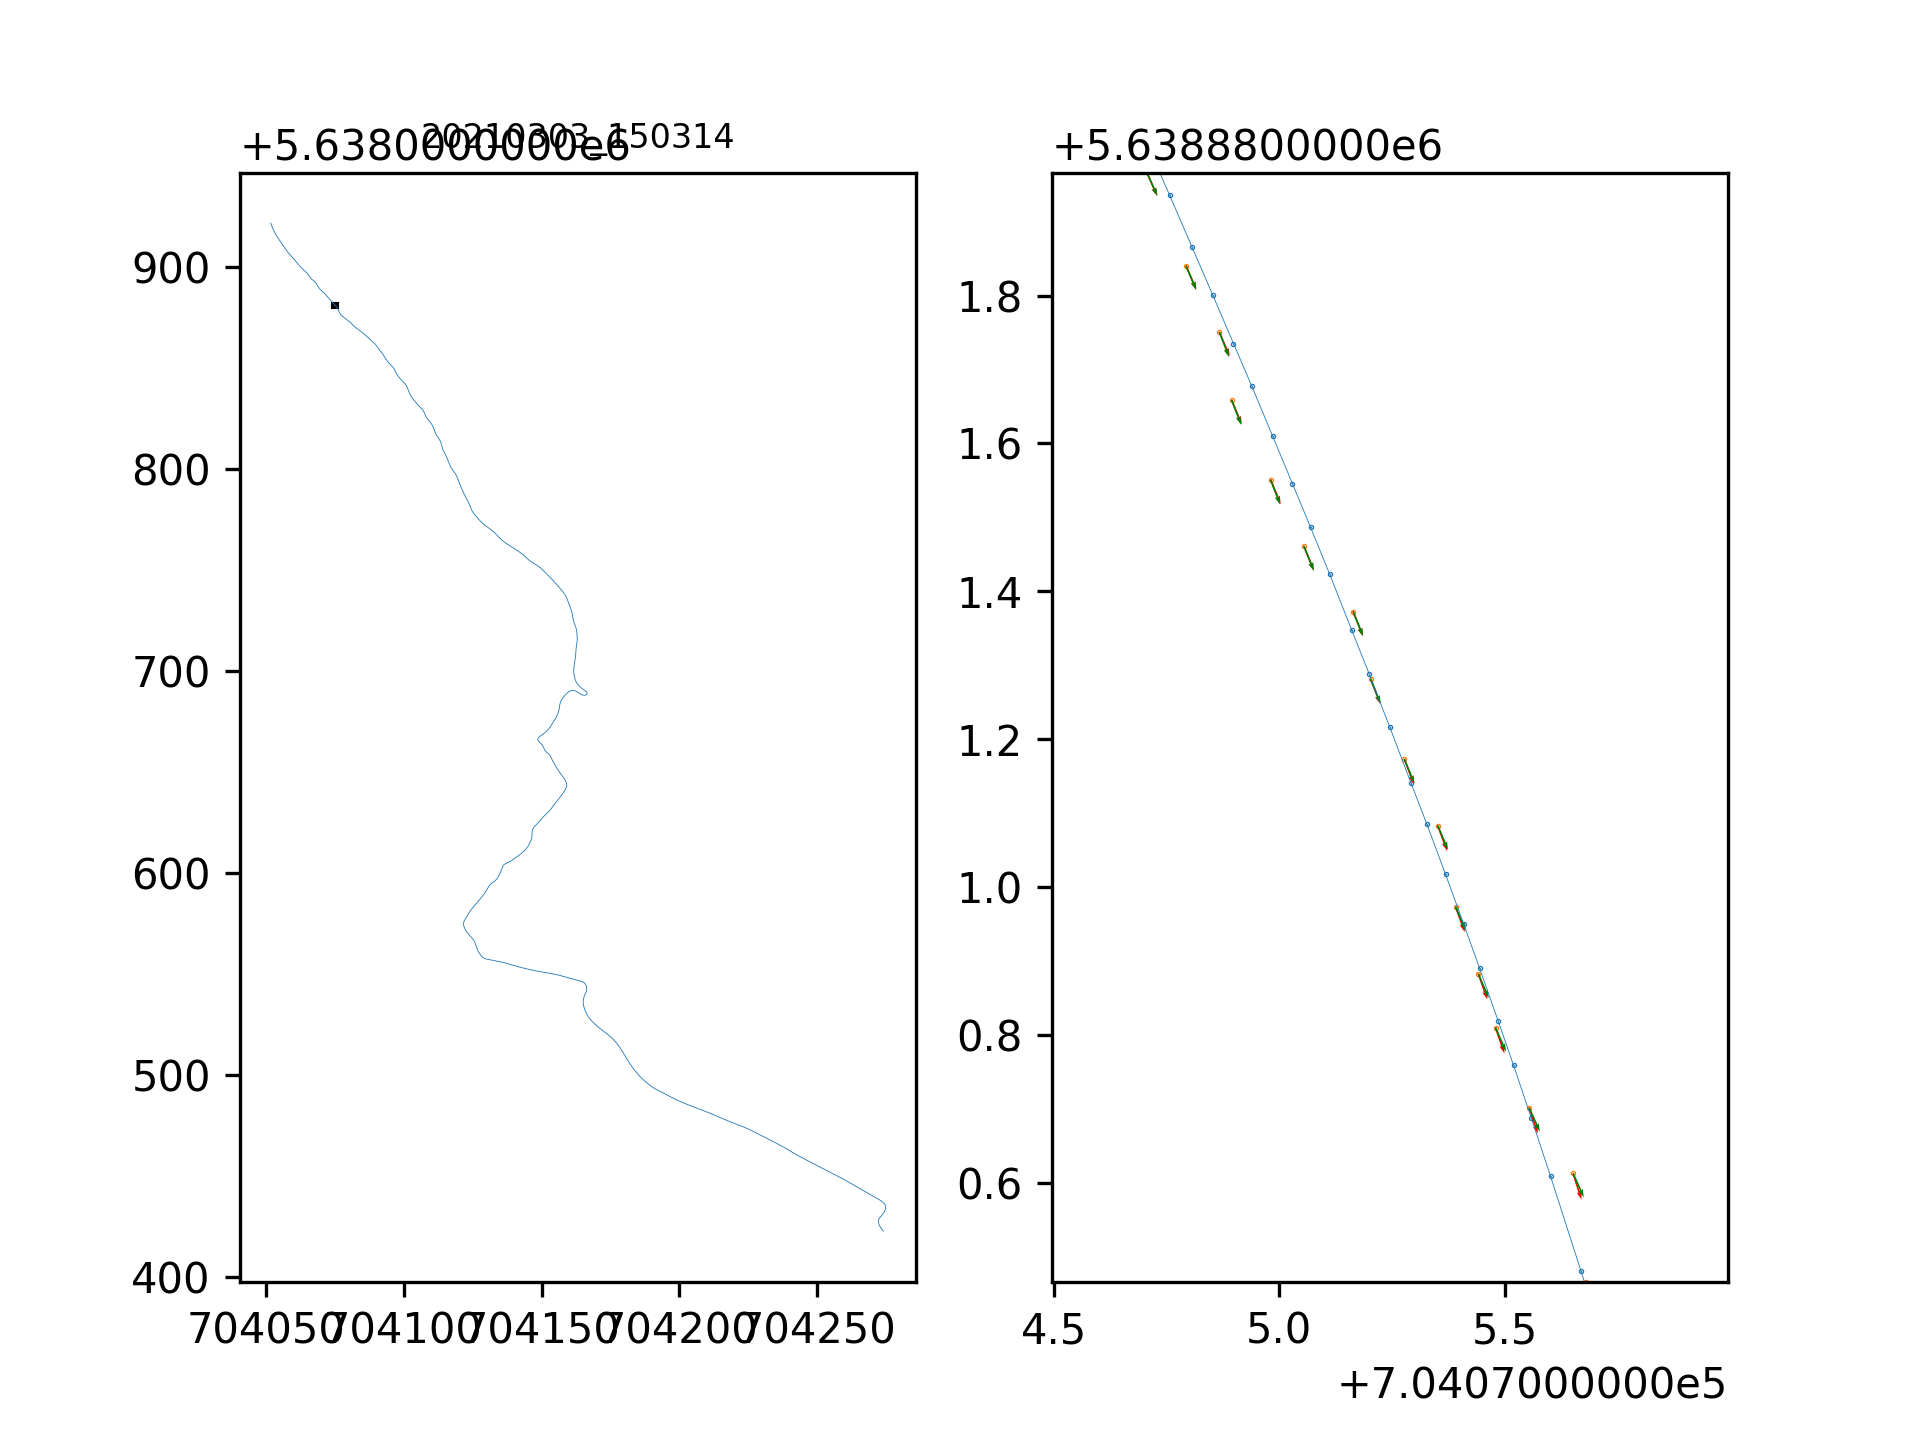
\includegraphics[width=\textwidth]{20210303_150314/frames_deg_1/frame_00809.png}
  \caption{\label{fig:frameEx1} Example of the cleaned data. left:
    full trajectory, right: enlargement of the area marked by the
    small rectangle in the left panel. Orange dots are original GPS
    positions, blue dots and line the interpolated trajectory, and red
    arrows GPS heading as well as green arrows showing the IMU
    heading. In this example they coincide very well (which is true
    most of the time).}
\end{figure}

\begin{figure}
  \includegraphics[width=\textwidth]{20210303_150314/frames_deg_1/frame_03579.png}
  \caption{\label{fig:frameEx2} Example of the cleaned data as
    above. In this example the headings diverge more (this is one of
    the most extreme examples on this trajectory).}
\end{figure}

Figures \ref{fig:frameEx1} and \ref{fig:frameEx2} show two individual
example frames of teh movie. In the former, the agreement of the headings is
excellent which is the case in most locations along the
trajectories. In the second example, there is a bit more
disagreement. However, this is much more rare and this is one of the
more extreme examples. It is worth noting that the IMU headings
after jump removal do not appear to degrade gradually along the
trajectory but appear to be quite reliable to the very end. This
suggests to me that they can be trusted to provide ground truth
along the trajectory (and more so than the GPS-derived headings
if there happens to be a discrepancy). Please note that I have here
displayed the heading arrows next to the original GPS waypoints
rather than the extrapolated points; this can be slightly confusing
where it is not obvious which extrapolated point corresponds to
which original waypoint.

\begin{figure}
  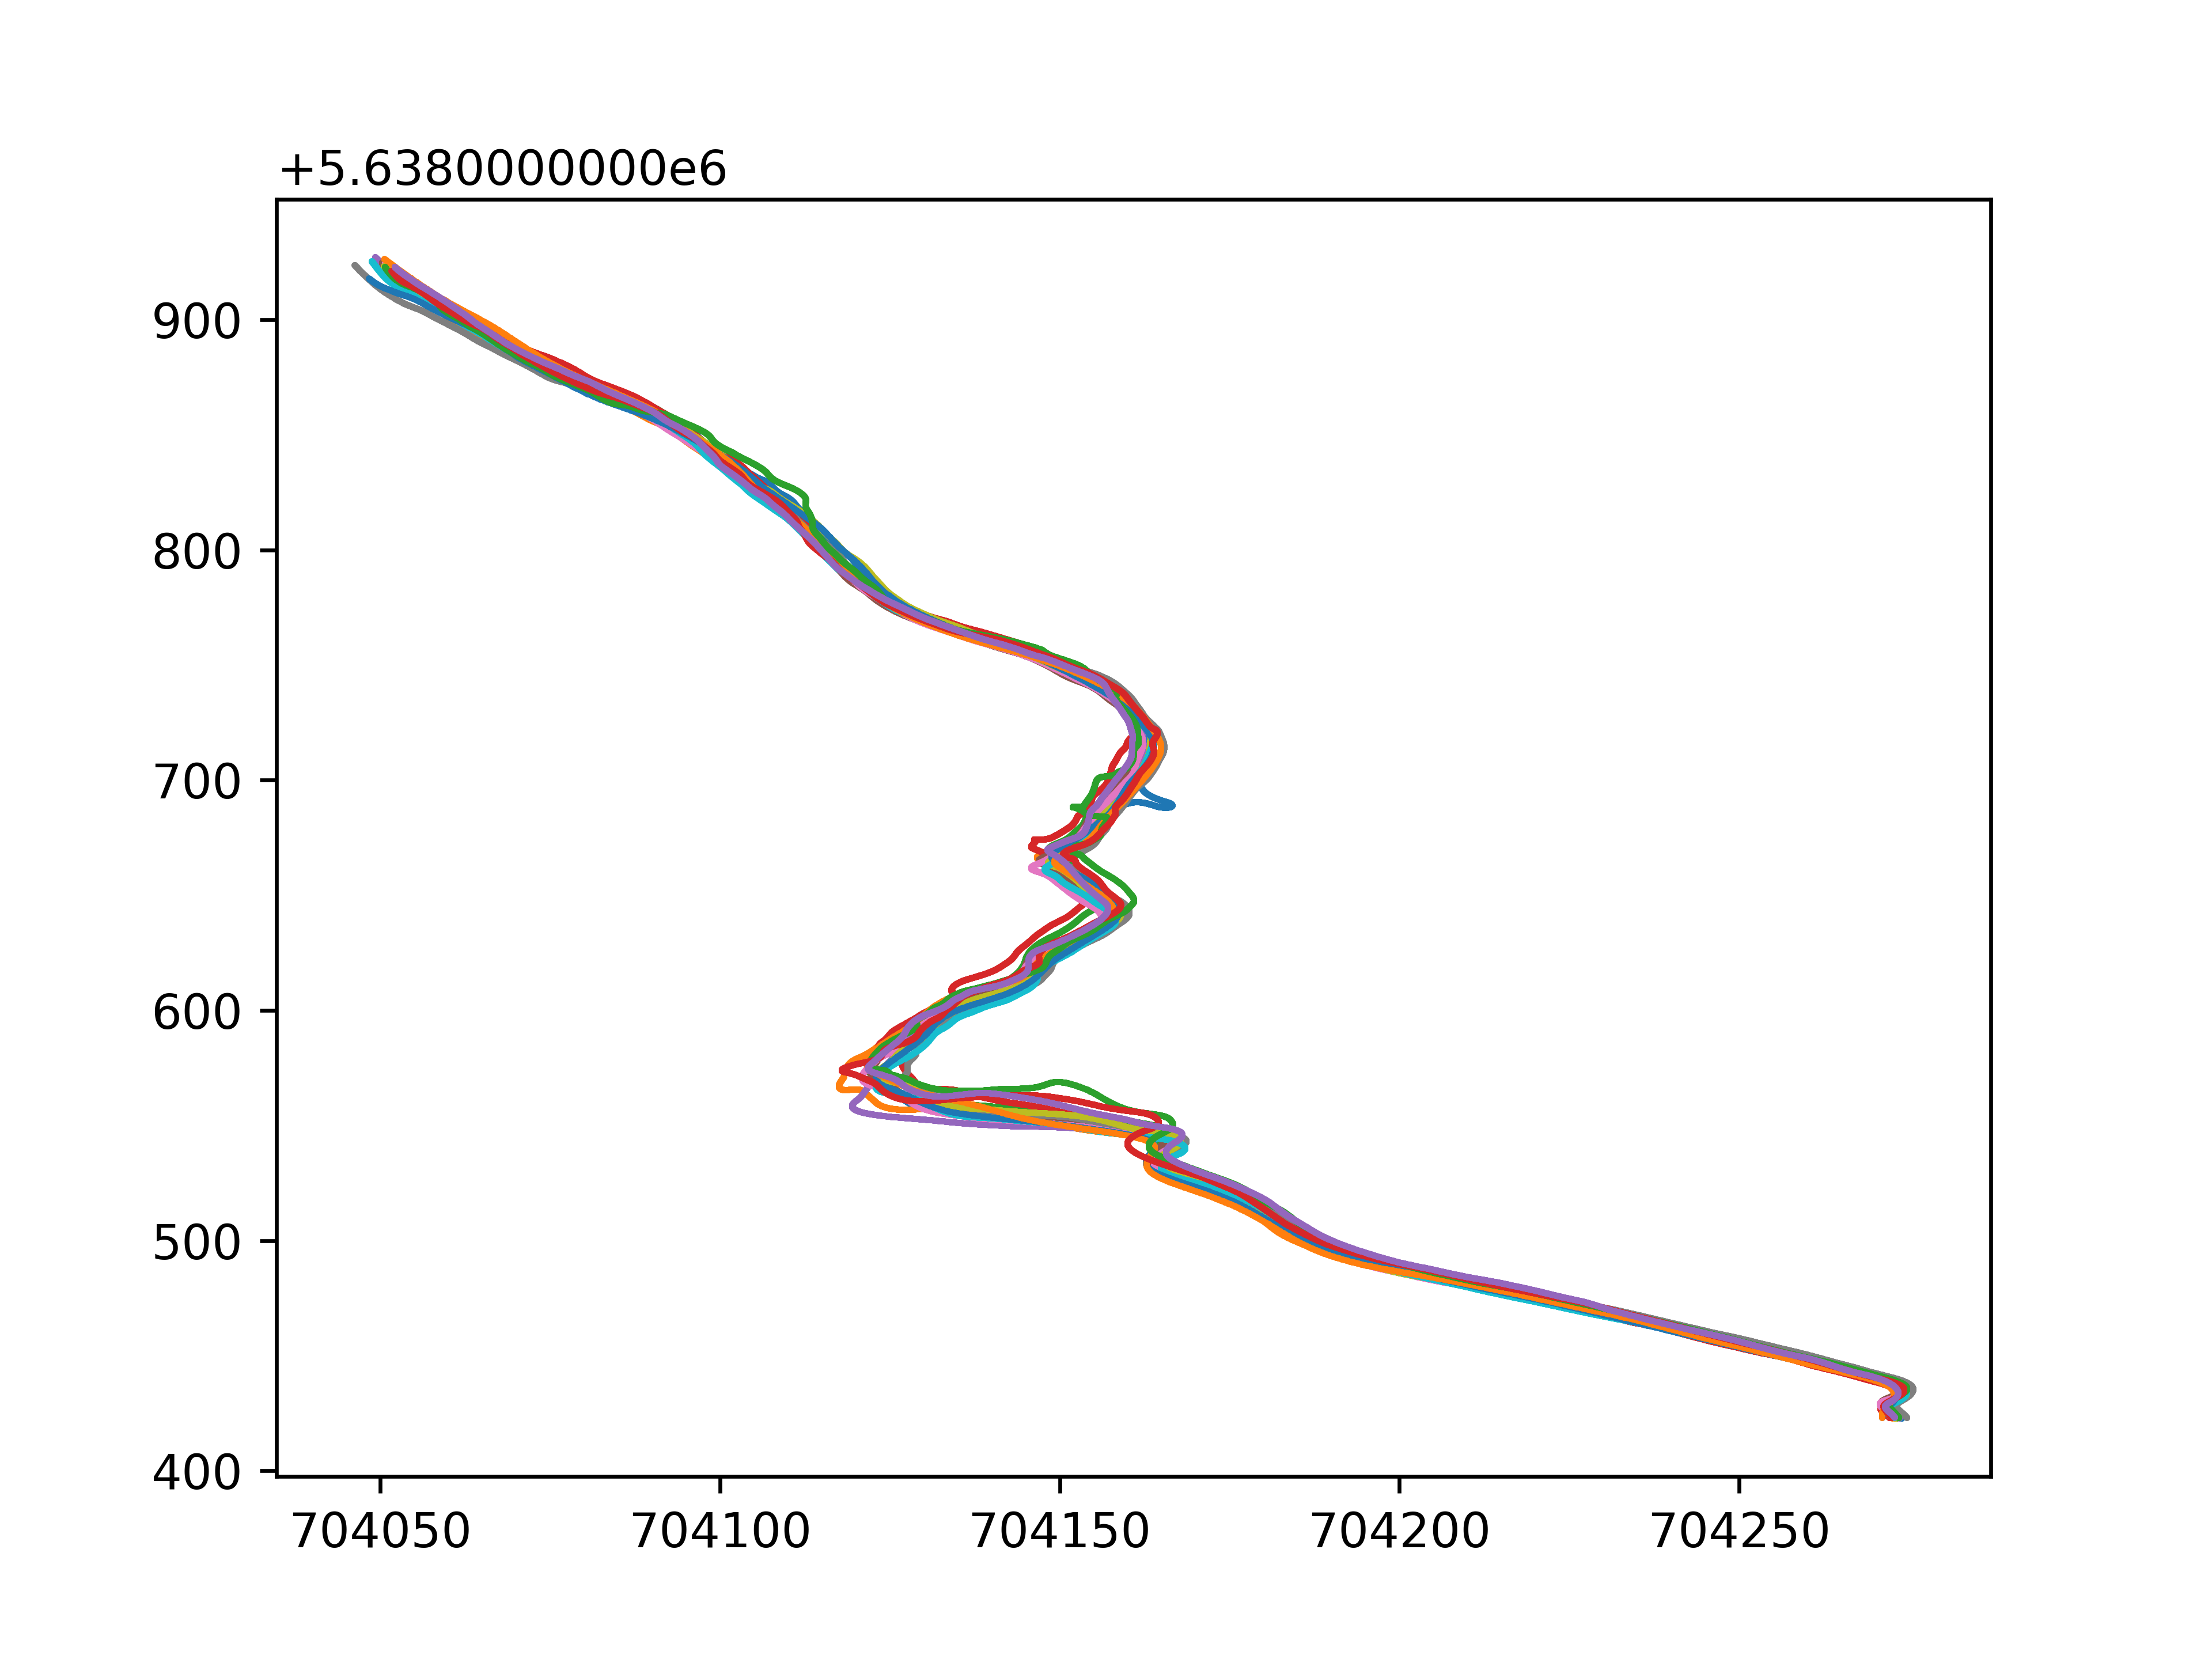
\includegraphics[width=\textwidth]{figures/fitted_trajectories_onepanel.png}
  \caption{\label{fig:fittedTraj1} Fitted trajectories plotted
    together. The spread of the original data is reproduced quite
    accurately.
    }
\end{figure}

\begin{figure}
  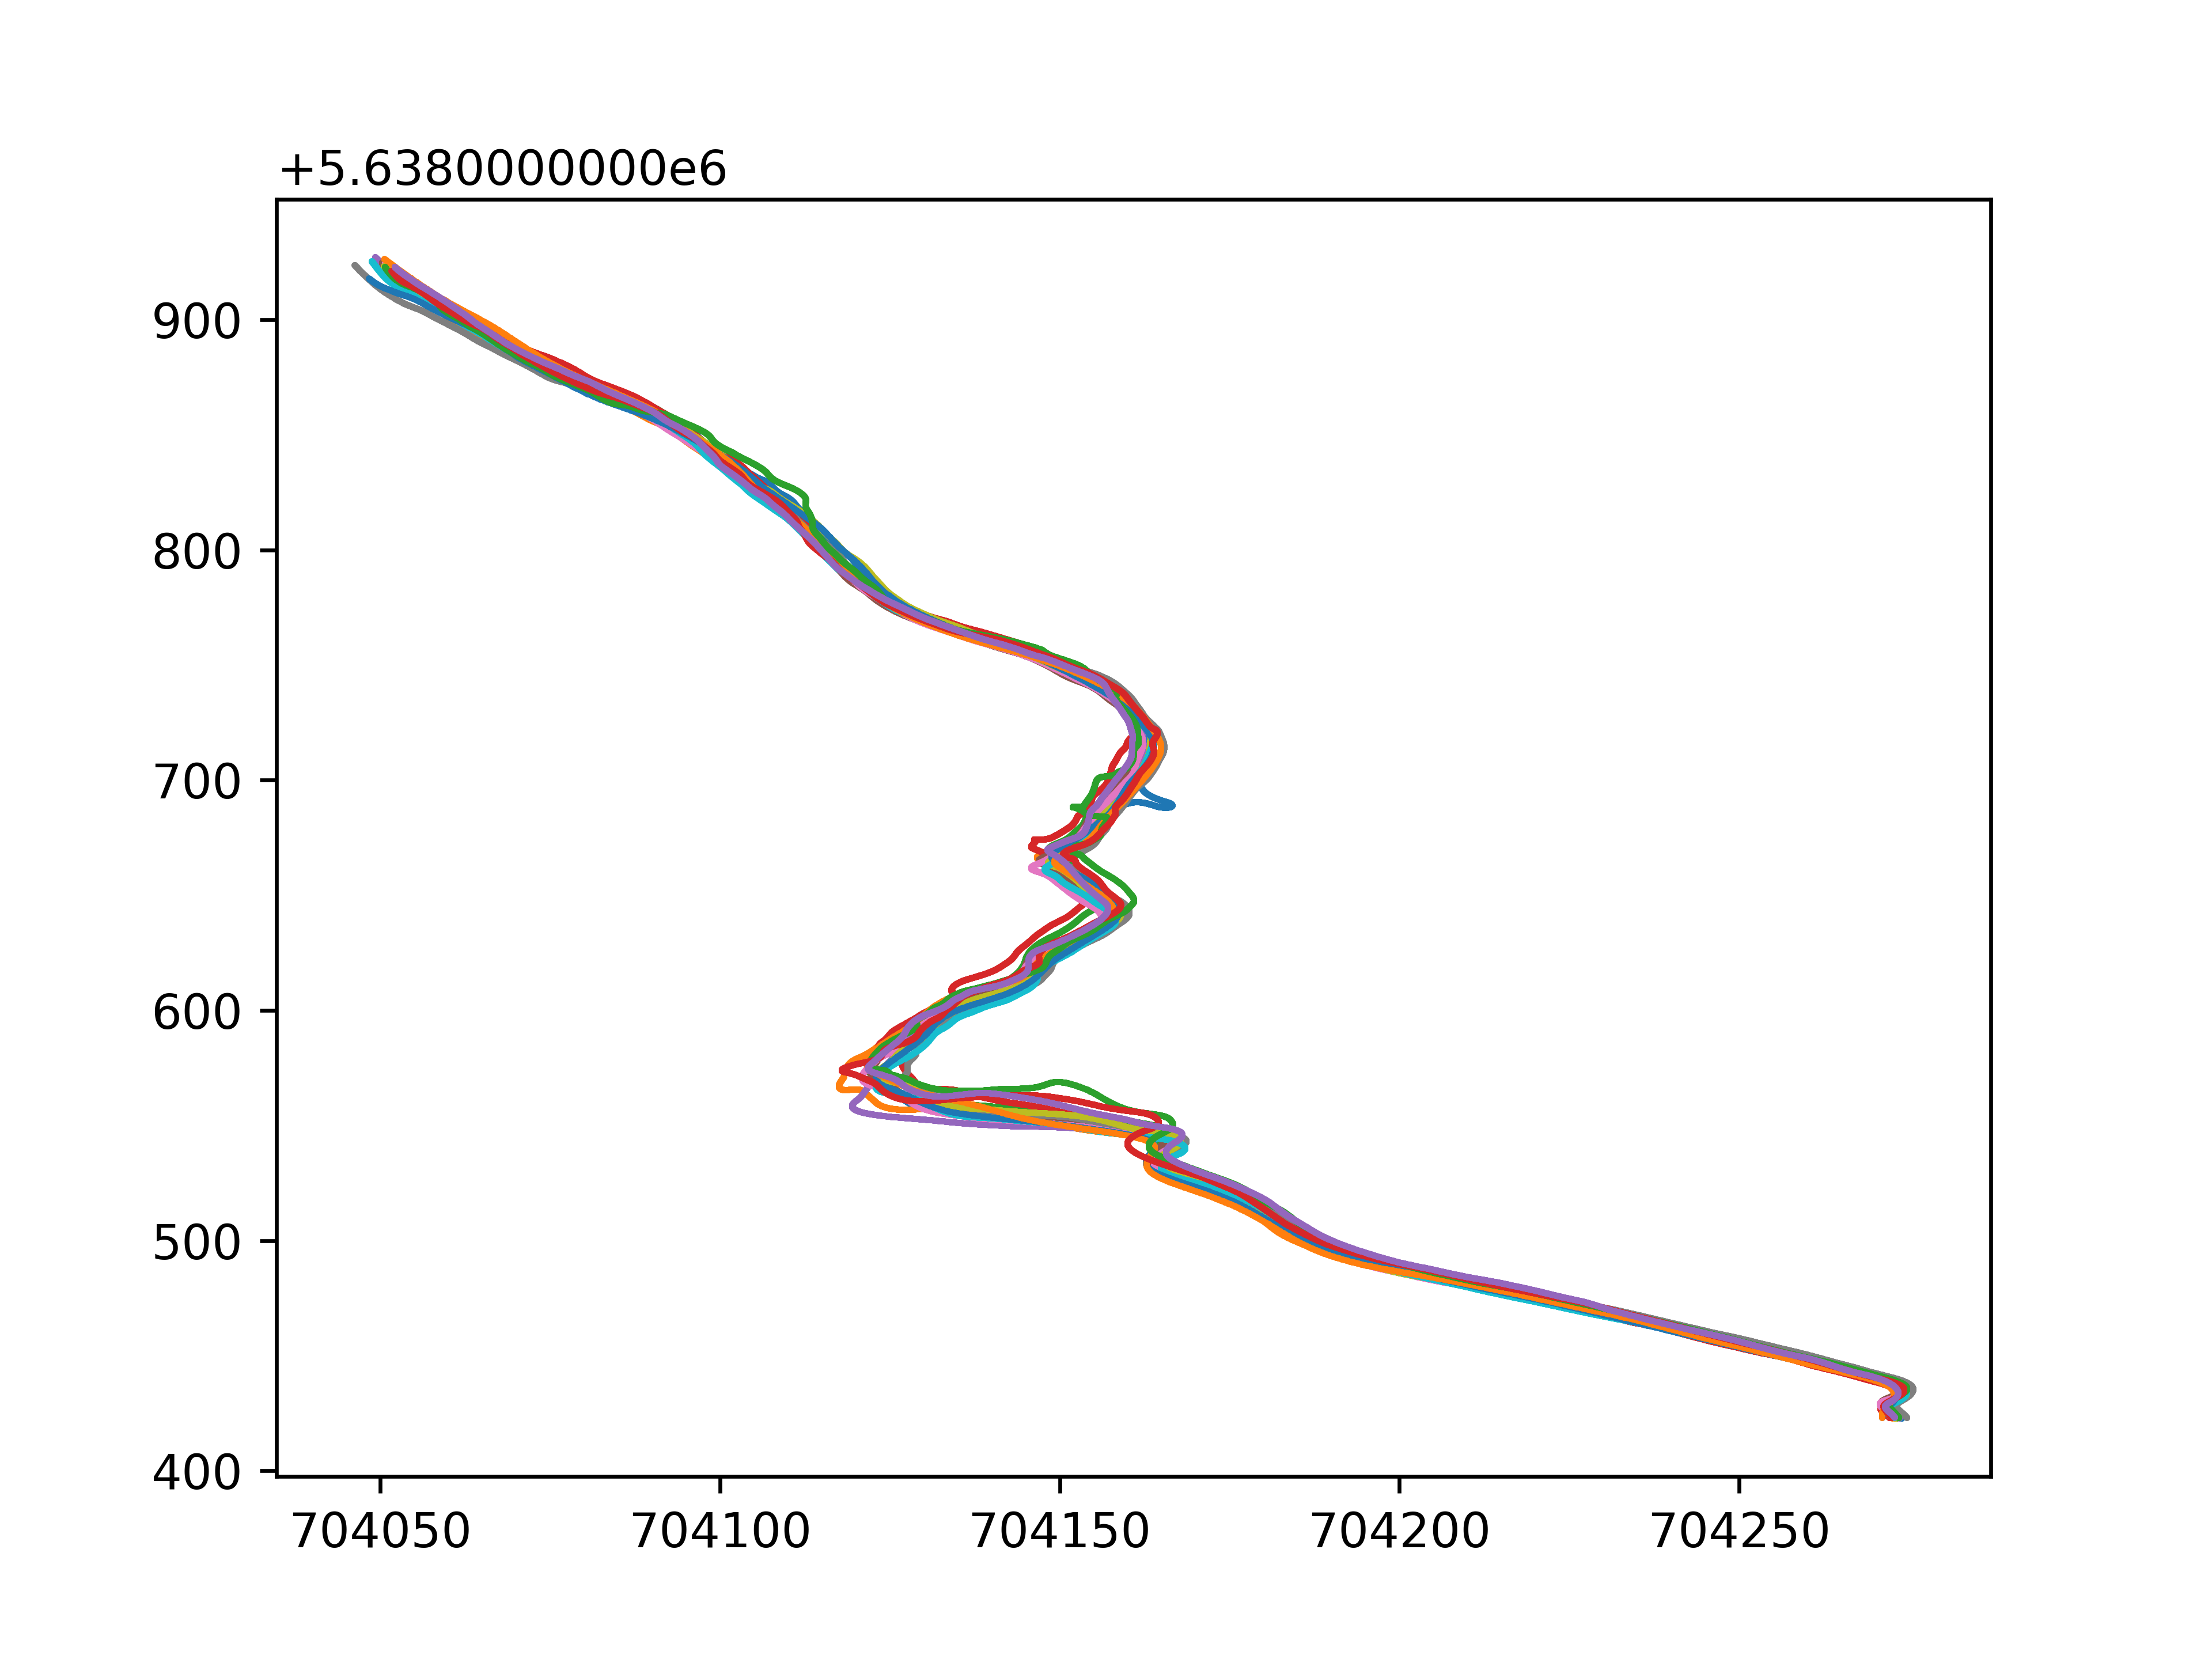
\includegraphics[width=\textwidth]{figures/fitted_trajectories_onepanel.png}
  \caption{\label{fig:fittedTraj2} Same as previous figure but with
    starting points collapsed onto the same point $(0,0)$.
    }
\end{figure}

Figure \ref{fig:fittedTraj1} shows the interpolated trajectories
altogether. The original shape and spread of the trajectories is
well-preserved (compare \ref{fig:procTraj1}).


When I went ahead and measured the pairwise distances of interpolated
trajectories with \verb+measure_0.py+, the trajectories ``as is'' were
closer together than if one makes the starting locations match (by
subtracting them), compare figure \ref{fig:fittedTraj1} and \ref{fig:fittedTraj2}. On average the summed distances were $26194.83$ (raw)
and $39009.99$ (same starting point).

As a fun exercise I used the IMU headings to reconstruct
trajectories. To lend a bit of a helping hand I used the interpolated
$x$ and $y$ coordinates to determine the size of stepes to make (the
speed in other words). Use \verb+reconstruct.py+. Figure \ref{fig:reconstruct} shows the results.

\begin{figure}
  \includegraphics[width=\textwidth]{figures/reconstructed_all.png}
  \caption{\label{fig:reconstruct} Trajectories reconstructed from IMU
    heading data (orange) compared to the interpolated trajectories
    (blue).}
\end{figure}

Even though there are obviously some discrepancies, overall the
trajectories are very similar, confirming once again that the IMU
heading data is quite accurate. There is a little bit of cheating
involved here through providing ``perfect speed information'' but that
does not take away from the fact that the heading data is overall mostly right.

\section{Examining images}
When observing odd trajectory bits in the generated trajectory movies,
it is unclear what might have happened. We, therefore, visually
inspected the camera footage of all datasets and identified obvious
abnormalities. These were essentially, the robot being still because
of a minor repair, or backing up briefly because stuck on
something. We manually identified the following segments: 
\begin{enumerate}
  \item
\verb+unwrapped_20210303_150314+ starts at 131; ends at tree 11304, no anomalies.
  \item
\verb+unwrapped_20210303_153749+ start at 125; ends at tree at about 10379 frames,
no anomalies.
  \item
\verb+unwrapped_20210308_122125+ starts at 151; ends at tree at about 9700 frames, no anomalies.
  \item
\verb+unwrapped_20210308_124836+ starts at 148; in between it looks like a loose cable or a thin
branch stuck on the robot; at 4209 strange maneuver to the left, back
out, continue, normal again from 4338; 5336 driving against a tree,
back out, continues route approx 5367; 8885 to 8906 slight stuck and
back out maneuver; 9044 to 9074 stuck and back up; ends at tree about
10333.
  \item
\verb+unwrapped_20210322_155544+ starts at 383; 5420: taking a left turn because
there are people in the way where he normally drives on the right of the
prominent tree; reaches the tree at 9851 but then drives off into
another direction without stopping
  \item
\verb+unwrapped_20210322_170743+ starts a 117; robot stuck at 7479, continues at
7608; reaches tree 9310, then drives off
  \item
\verb+unwrapped_20210414_151116+ start at 127; reaches tree 9157, then
drives off
  \item
\verb+unwrapped_20210420_135721+ start at 339; 6294 to 6326 robot goes
back and forth; same 6759 to 6781; 7138 to 7163; 7174 to 7209; 7834 to
7853; 8256 to 8280; 8371 to 8389; reaches tree at 10026 but the last
bit of the route looked visually as if it was too far to the left!
  \item
\verb+unwrapped_20210420_141940+ start at 86; reaches tree 9410 then
takes off.
  \item
\verb+unwrapped_20210422_134815+ start at 135; doesn't go to the tree!
Instead to a different stopping point where it stands still for quite a
while ...
  \item
\verb+unwrapped_20210426_162152+ starts at 50; reaches tree 3673 -
very fast driving on this one!
  \item
\verb+unwrapped_20210426_164219+ starts at 69; frames stop prematurely
at 3129; this is in agreement with the csv files.
  \item
\verb+unwrapped_20210511_151514+ starts at 199; 1377 to 1414 back and
forth; from about frame $3635$ to $3925$ the robot stood still while
Norbert was fixing the robot (apparently something had fallen off);
reaches tree 10357 
  \item
\verb+unwrapped_20210511_153933+ starts at 112; reaches tree at 10099,
then drives off
  \item
\verb+unwrapped_20210525_141844+ starts at 154; stops at tree 8764
rest is irrelevant.
\end{enumerate}

The manual exclusions were coded into a new script
\verb+zero_chop_visual.py+ which operates on the data tables in the
\verb+unwrapped_*+ directories. There are
\verb+fit_trajectories_visual.py+ and \verb+correct_heading_visual.py+
scripts that essentially recapitulate the workflow above for the
manually cut data. The results are essentially of similar quality,
with some of the obvious artifacts removed.

The \verb+make_movie_frames_visual.py+ script improves on teh previous
script by including the camera feed into the movie so that one can now
see the reconstructed trajectories and headings in conjunction with
the views from the camera.

There is also a \verb+reconstruct_visual.py+ and
\verb+reconstruct_visual_greedy.py+ script. The former recapitulates
\verb+reconstruct.py+ but on the manually trimmed data sets. The
\verb+_greedy+ version is trying to reconstruct the trajectory based
on IMU data but rather than using the distance travelled between
corresponding points on the fitted trajectory, it is determining the
distance travelled that will minimise the distance of the IMU
trajectory point to the corresponding fitted trajectory point. I named
it greedy, as it is optimising this in a greedy way from the start of
the trajectory and this local minimisation of divergence between
trajectories can of course lead to larger divergences later on.

I have also tried a global optimisation using the Nelder-Mead simplex
alogrithm on the vector of all distances travelled but it appears that
this probem might be too high-dimensional/ the optimisation to be too
slow to be useful.



\section{Appendix}
To make the movies I used
\begin{verbatim}
ffmpeg -framerate 10 -pattern_type  glob -i "frame_*.png" output.mp4
\end{verbatim}

\end{document}
